%\bibliographystyle{ieeetr}
%\bibliographystyle{splncs}
%\bibliographystyle{elsart-harv}
%\bibliographystyle{ipsjunsrt-e}
\bibliographystyle{ieicetr}




\Chapter{かけると便利なスクランブル --- ランダム射影 ---}


\Section{原理}

ランダム射影(random projection)は,乱数で作った行列$\mtr R$による
線形写像である.
$d_x$次元ベクトル$\vec x\in\mathbb{R}^{d_x}$から
$d_p$次元ベクトル$\vec p\in\mathbb{R}^{d_p}$へのランダム射影は
\begin{equation}
%\mbox{\ RandomProjection(\vec x\|\mtr R)}\defas
\vec p=\mtr R\vec x
\end{equation}
と書ける.
$\vec x$は$d_x$次元ベクトルで,
実数の成分を持つどんなベクトルでも構わない.
$\vec p$は$d_p$次元ベクトルである.
$d_x$次元ベクトルを$d_p$次元へ写像するランダム行列$\mtr R$は,
サイズが$d_p\times d_x$の行列で,次のように書き表すことができる.
\begin{equation}
 \mtr R=\bmatrix{ccc}{
r_{11} & \cdots & r_{1d_x} \\
\vdots & \ddots & \vdots \\
r_{d_p1} & \cdots& r_{d_pd_x}
}
=\bmatrix{c}
{\vec r_1^\top\\
\vdots\\
\vec r_{d_p}^\top}\in\mathbb{R}^{d_p\times d_x}.
\end{equation}
行列$\mtr R$の第$i$行は,横に転置した$d_x$次元ベクトル$\vec r_i^\top$である.
$d_p$本の$d_x$次元ベクトル$\vec r_i$($i=1,\dots,d_p<d_x$)は,
図\ref{fig:RP}に示すように,
$d_x$次元空間$\mathbb{R}^{d_x}$における$d_p$次元の部分空間を張る.
よって,行列$\mtr R$によるランダム射影は,
任意の$d_x$次元ベクトル$\vec x$(図中の$\vec x^{(1)}$や$\vec x^{(2)}$)を,
この部分空間に正射影して$d_p$次元ベクトル$\vec p$を作る演算になっている.
\begin{equation}
% \vec p=\mtr R\vec x=[\vec r_1^\top\vec x,\dots,\vec r_{d_p}^\top\vec x]^\top
\vec p=\mtr R\vec x=\bmatrix{c}{
\vec r_1^\top\vec x\\
\vdots\\
\vec r_{d_p}^\top\vec x}\in\mathbb{R}^{d_p}
\end{equation}

\begin{figure}[hb]
\setlength{\unitlength}{1cm}
\begin{center}
%\fbox{
\begin{picture}(5,4.5)
%\put(0,0){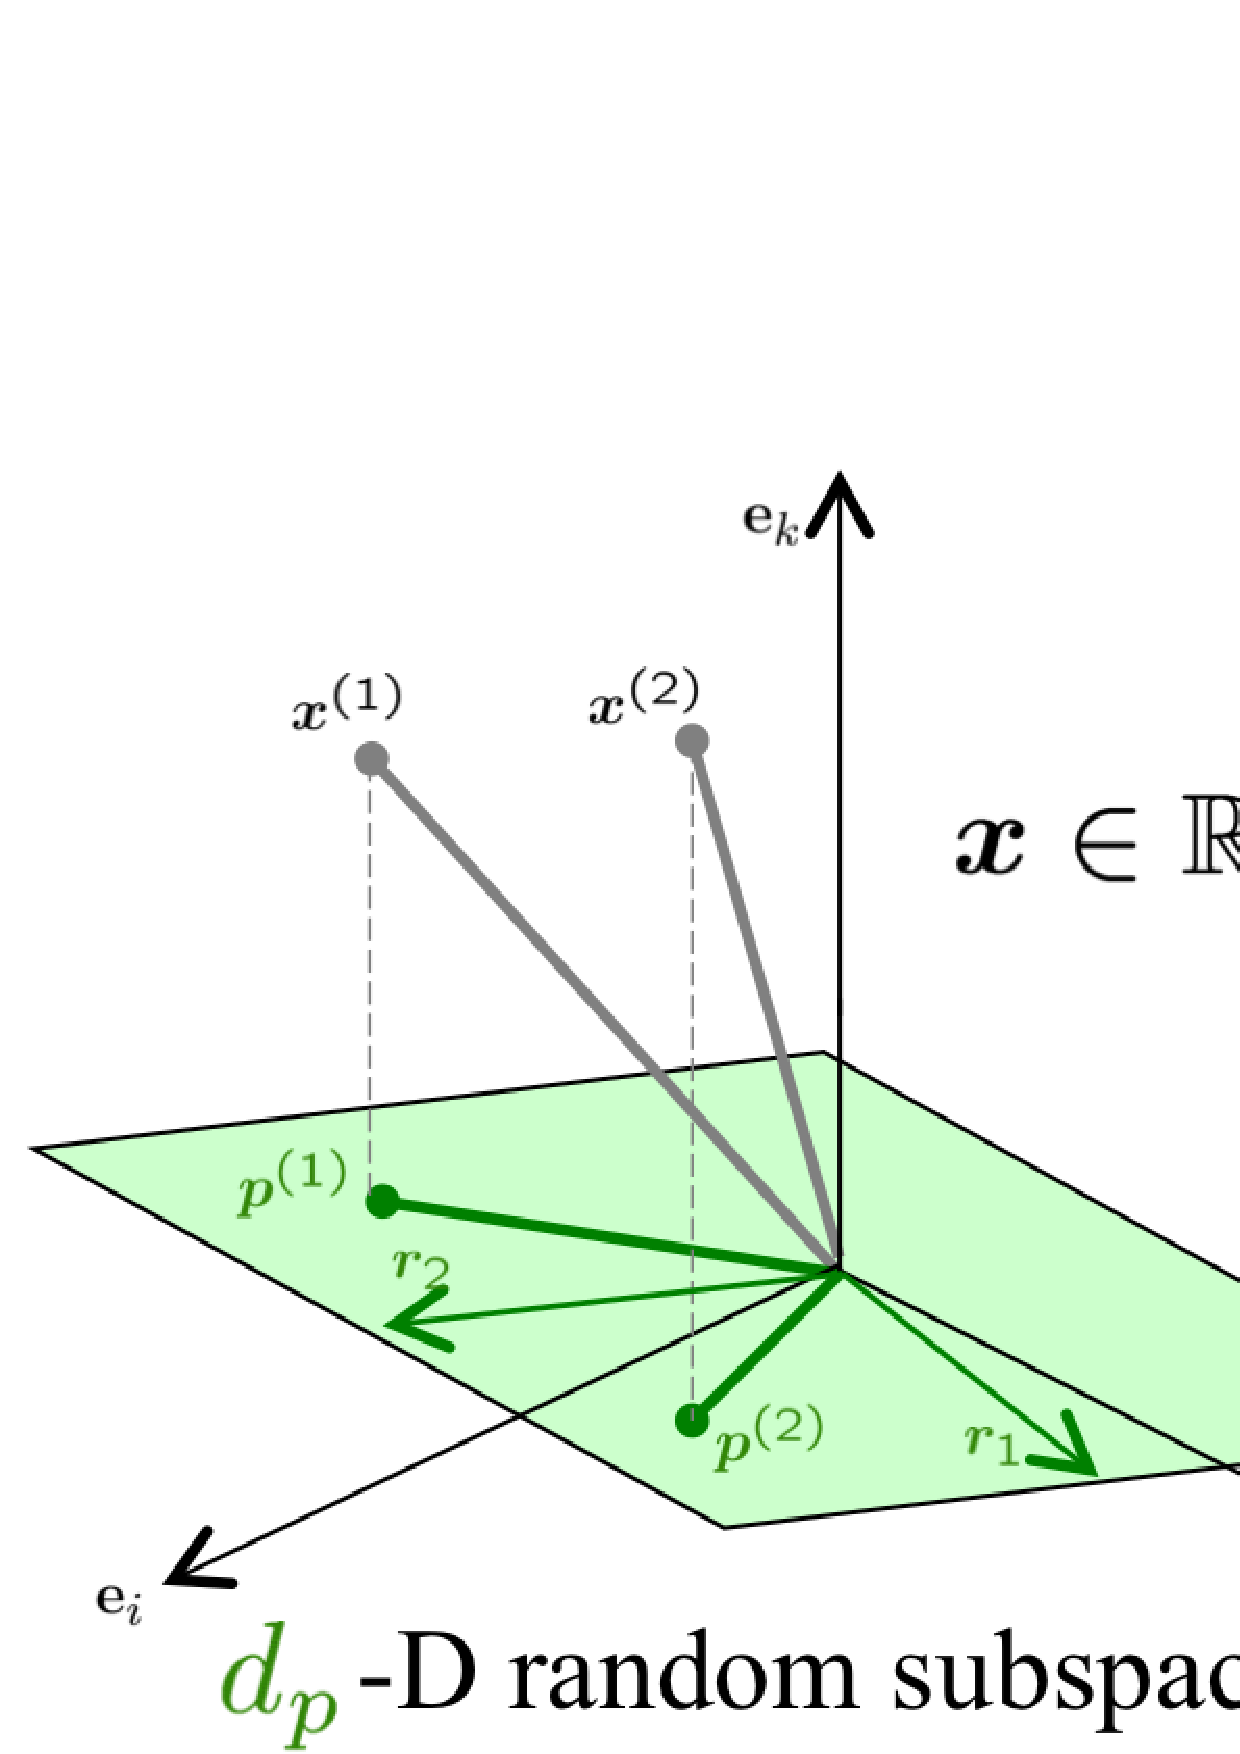
\includegraphics{RP.pdf}}
\put(0,0){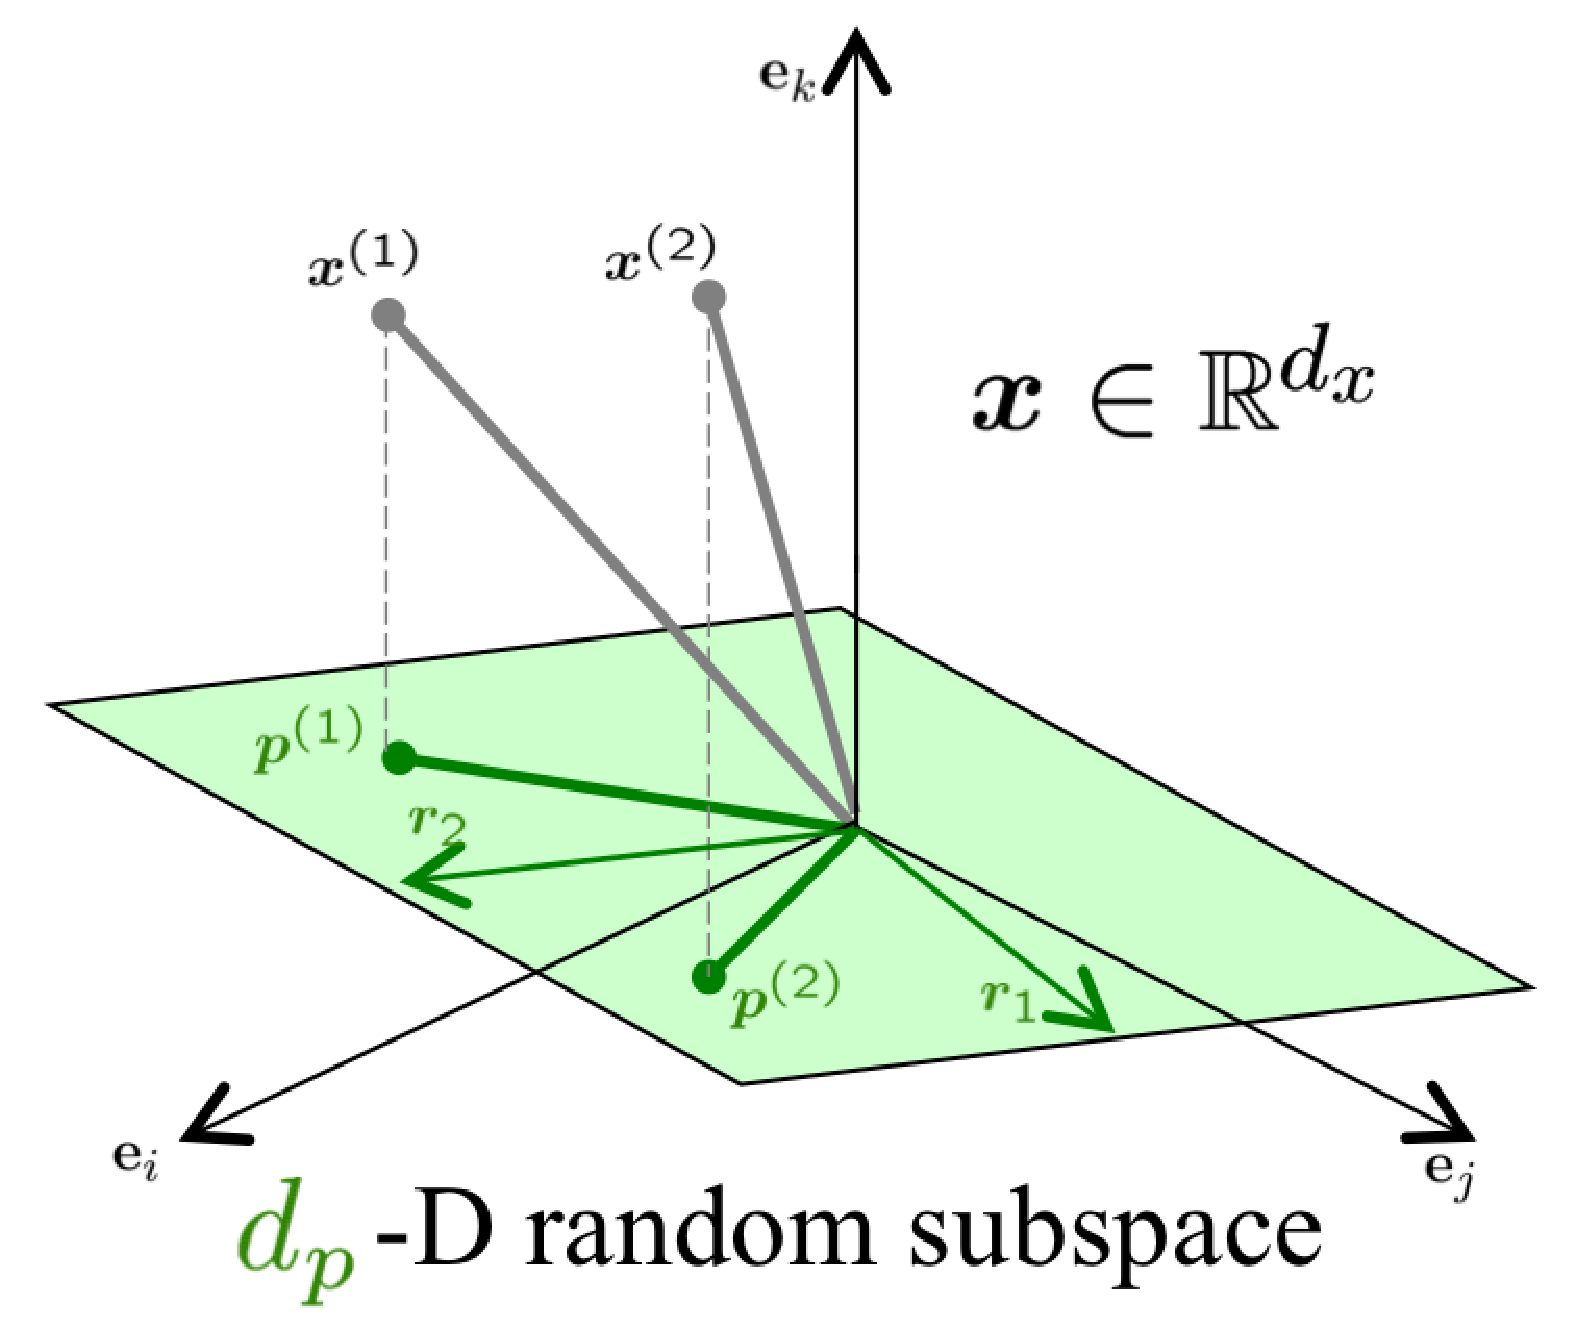
\includegraphics[height=4cm]{RP.eps}}
%\centerline{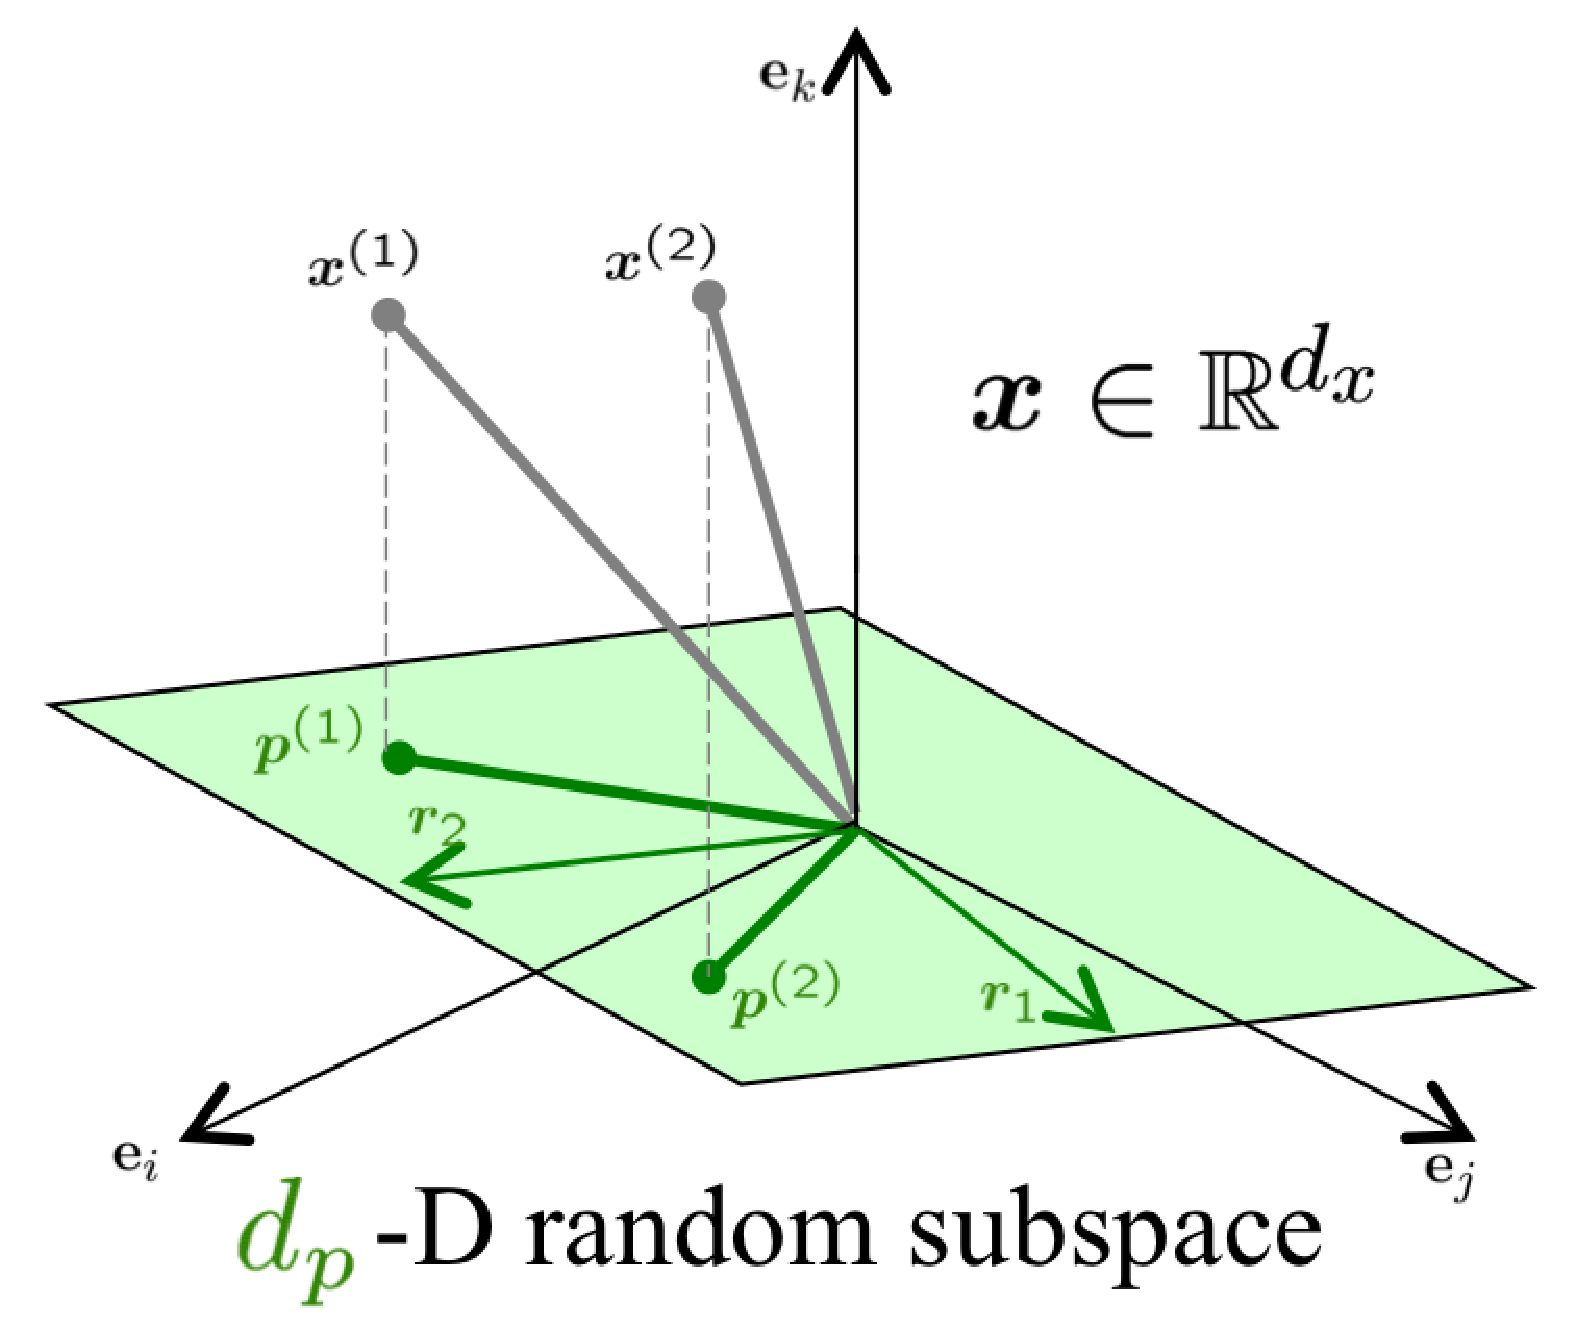
\includegraphics[height=4cm]{RP}}
\end{picture}%}
 \caption{$\vec x\in\mathbb{R}^{d_x}$から$\vec p\in\mathbb{R}^{d_p}$への
ランダム射影.}
\label{fig:RP}
\end{center}
\end{figure}

例えば,平均ゼロ,分散$1/d_p$の正規分布から
ランダム行列$\mtr R$を生成するとしよう.
すると,
$d_x$次元ベクトルで表された
データの集合$X\subset\mathbb{R}^{d_x}$を
ランダム射影した低次元データ集合
$P=\{\vec p\;|\;\vec p=\mtr R\vec x,\vec x\in X\}\subset\mathbb{R}^{d_p}$
は,$X$の様々な性質を高い確率で近似的に保持することが知られている\cite{Vempala04}.
例えば,2本の
ベクトル$\vec x^{(i)},\vec x^{(j)}\in X$をランダム射影した
ベクトルをそれぞれ$\vec p^{(i)},\vec p^{(j)}\in P$とする.
\[
\vec p^{(i)}=\mtr R\vec x^{(i)},\quad \vec p^{(j)}=\mtr R\vec x^{(j)}%,
%\quad\forall \vec x^{(i)},\vec x^{(j)}\in\mathbb{R}^{d_x}.
\]
すると,$\vec p^{(i)}$のノルムは$\vec x^{(i)}$のノルムの良い近似値になる.
同様に,2点$\vec x^{(i)},\vec x^{(j)}\in\mathbb{R}^{d_x}$の間の
距離や内積も高確率で近似的に保存される\footnote{%
$\approx$は近似的に等しいの意味.`≒'の記号を使うのは日本だけらしい(?)}.
\begin{eqnarray}
\|\vec p^{(i)}\|_2 &\approx& \|\vec x^{(i)}\|_2,\\
||\vec p^{(j)}-\vec p^{(i)}||_2 &\approx& ||\vec x^{(j)}-\vec x^{(i)}||_2,\\
{\vec p^{(j)}}^\top\vec p^{(i)} &\approx& {\vec x^{(j)}}^\top\vec x^{(i)}
\end{eqnarray}

ランダム射影で近似的に保存される性質を
図\ref{fig:RP properties}に列挙する.
計量,多様体の構造,2クラス間のマージン,核関数,
主成分等が保存されることが既に解明されている.
\begin{figure}[hb]
\setlength{\unitlength}{1cm}
\begin{center}
%\fbox{
\begin{picture}(14,8)
%\put(0,0){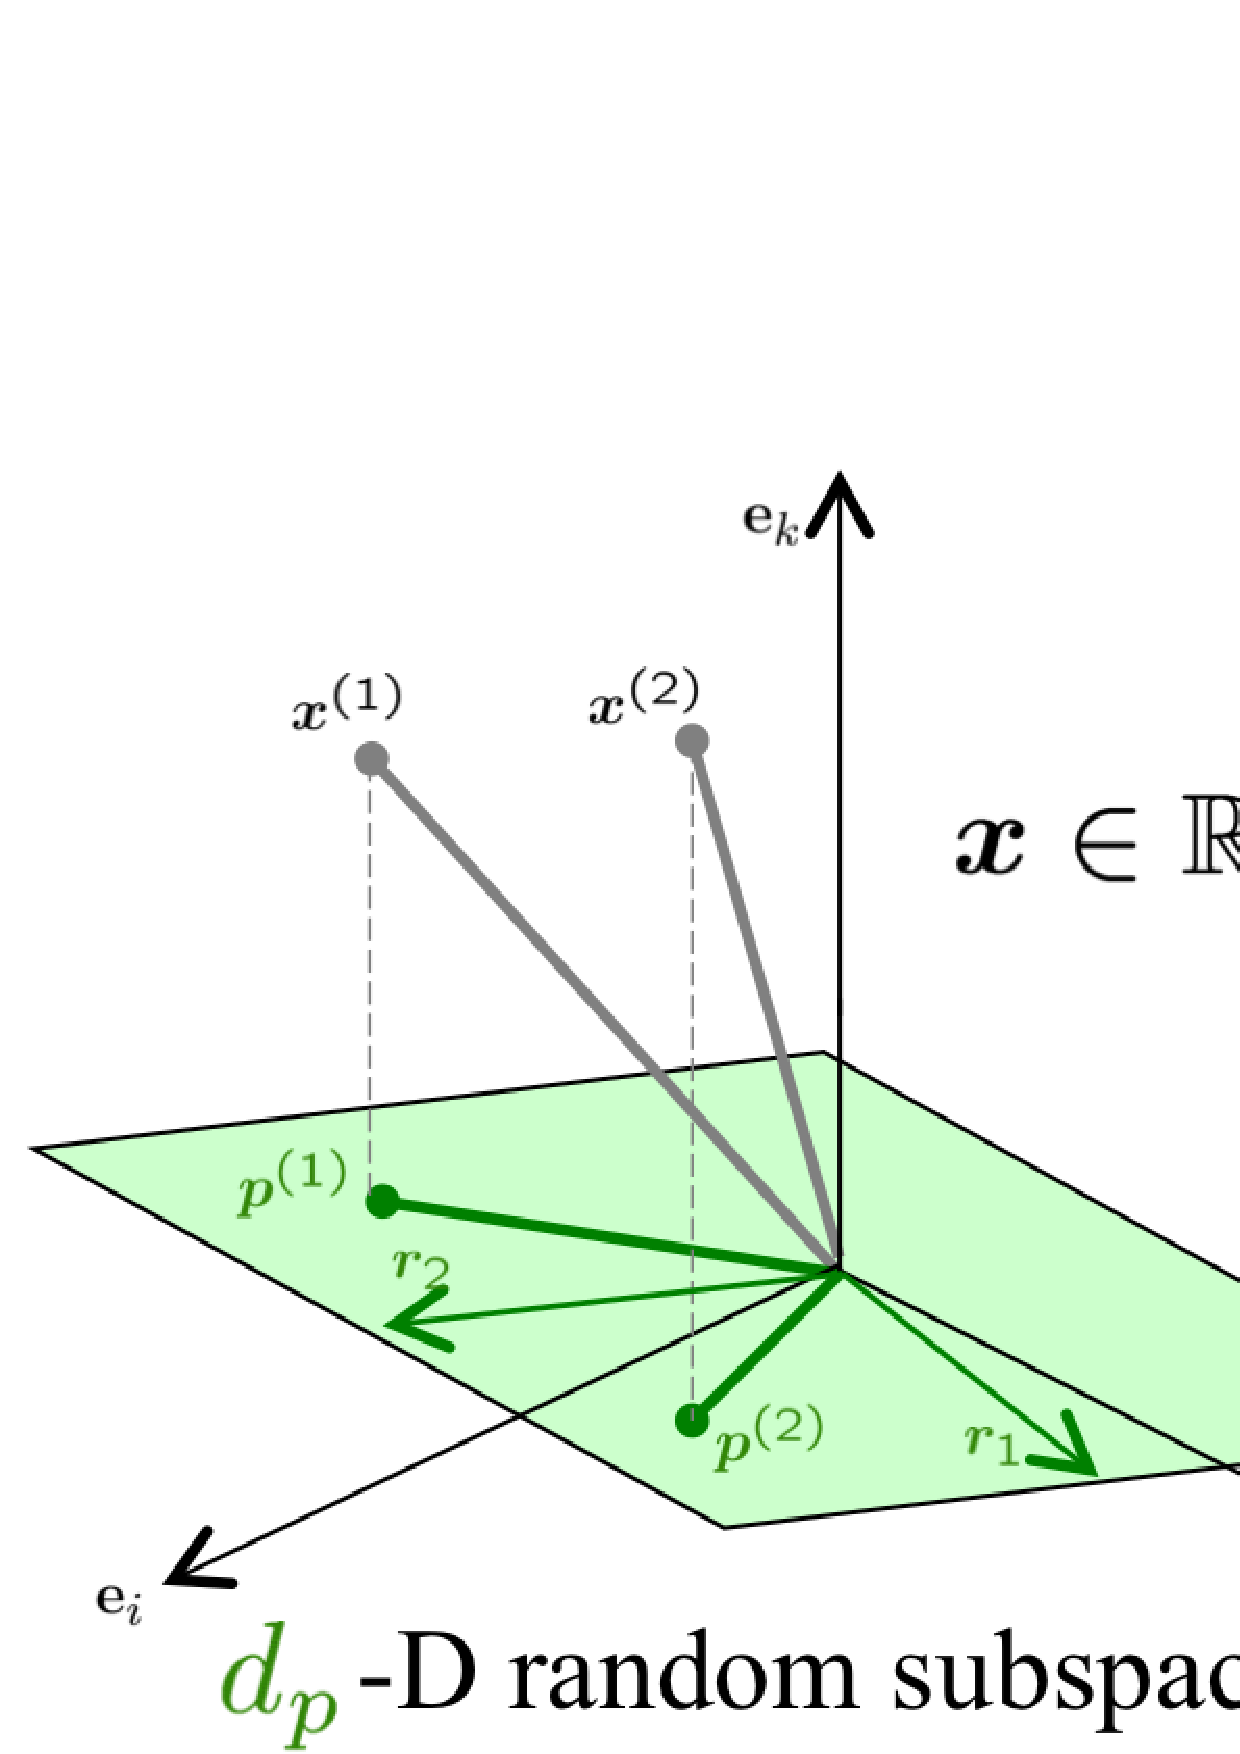
\includegraphics{RP.pdf}}
\put(0,-0.5){\includegraphics[height=8cm]{RPp.eps}}
%\centerline{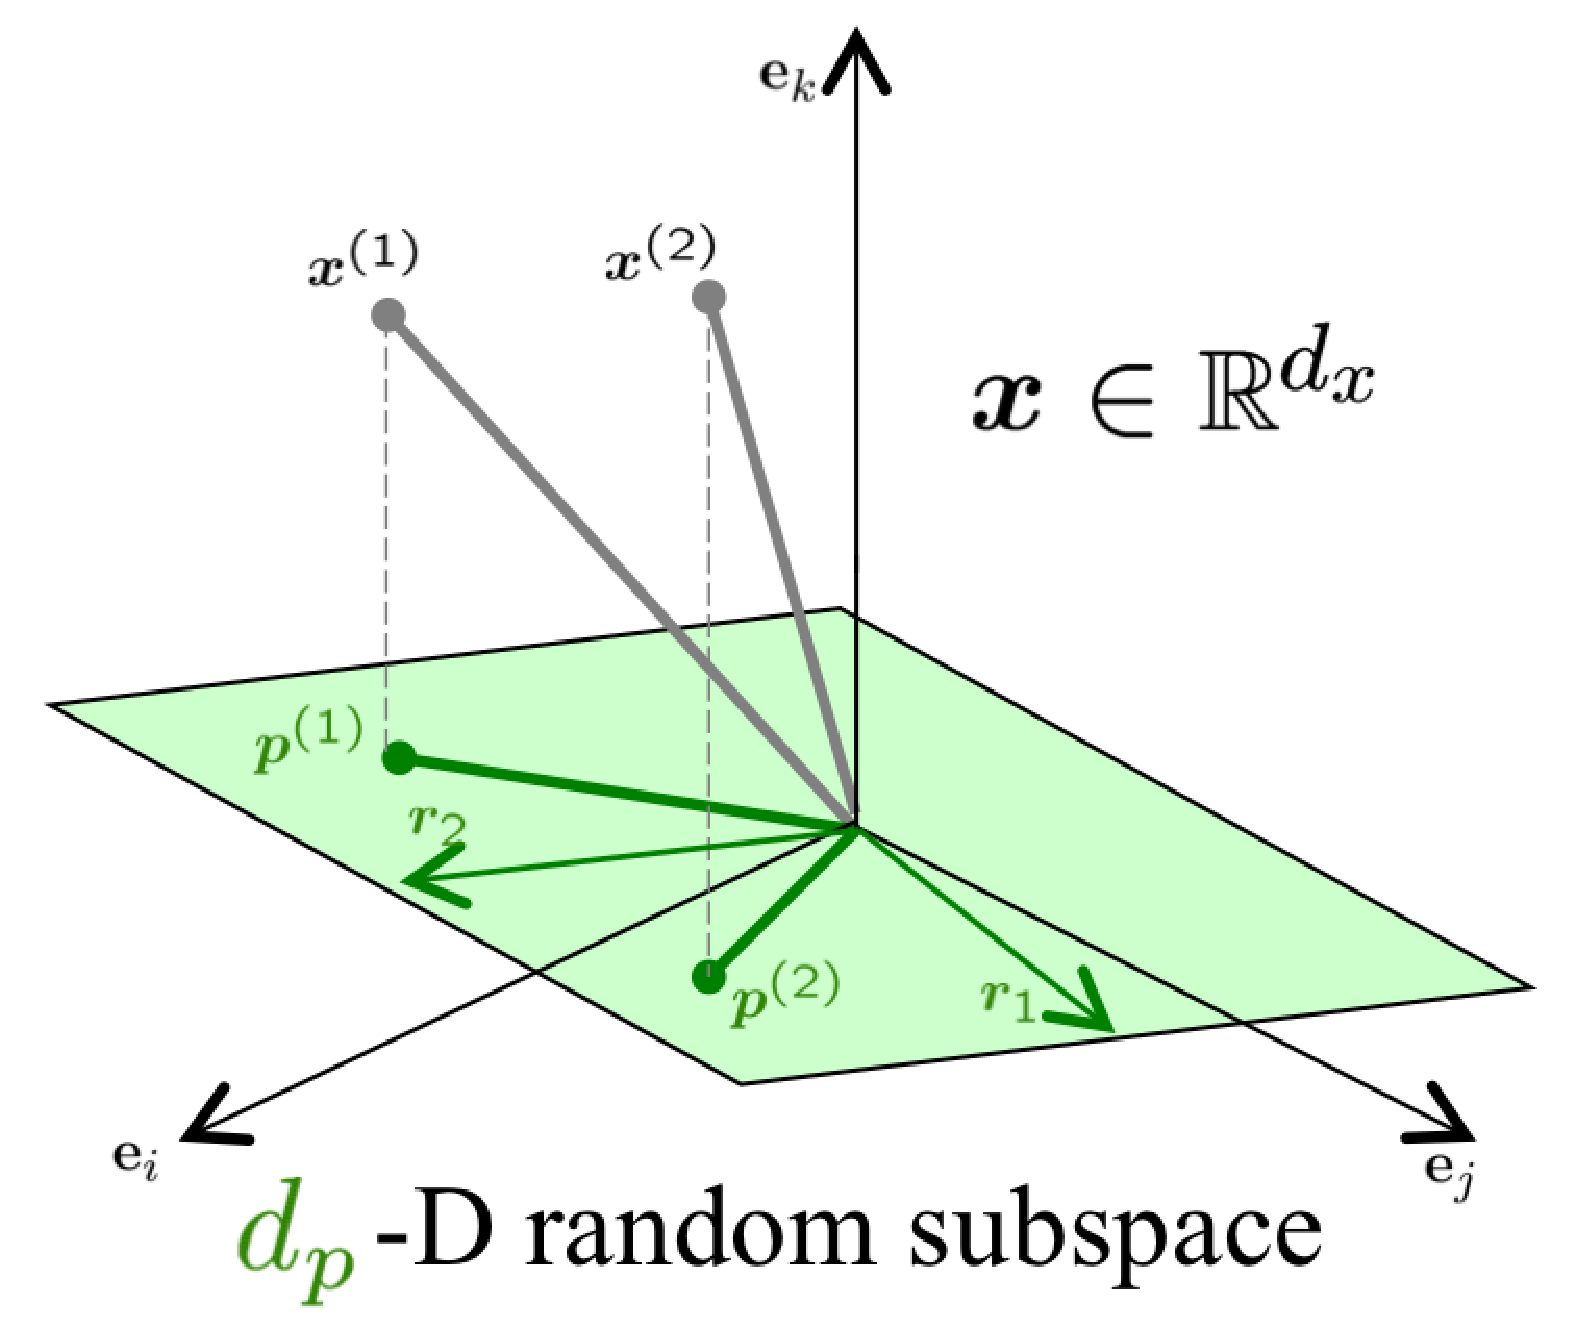
\includegraphics[height=4cm]{RP}}
\end{picture}%}
\end{center}
 \caption{What preserved after random projection.}
\label{fig:RP properties}
\end{figure}


パターン認識(pattern recognition; PR)や機械学習(machine learning; ML)と
呼ばれる研究分野では,
データの特徴を高次元ベクトルで表して分類や予測を達成する
様々な解析手法が設計されている.
内積や距離は,2つのデータの間の類似性・非類似性を測った量と見なせる.
そのような量がランダム射影で近似的に保存されるということは,
低次元データ集合$P$を使って高次元データ集合$X$を解析できることを意味している.
つまり,ランダム射影を使ってPR/MLの計算コストを低減できる
\footnote{ただし,ランダム射影自体の計算コストが問題にならないことが前提である.}.



\Section{試してみよう}

\lstset{language=Matlab}
\lstset{basicstyle={\tt},identifierstyle={\bfseries},keywordstyle={\bfseries}}
\lstset{tabsize=2,showstringspaces=false}
\lstset{commentstyle={\color[rgb]{0,0.5,0}}}
\lstset{flexiblecolumns=true}
\lstset{classoffset=1,breaklines=true,morecomment=[l]{//}}
%\lstset{columns=[l]{fullflexible}}
%\lstset{numbers=left,stepnumber=1,numberstyle={\scriptsize},numbersep=4ex}
\lstset{frame=tBlR,rulecolor={\color[gray]{0.75}},rulesepcolor={\color[gray]{0.75}}}
\lstset{framesep=2ex}
\lstset{xleftmargin=8ex,xrightmargin=16ex}
%\lstset{backgroundcolor={\color[rgb]{1,1,0.95}}}

\paragraph{ノルムを比べてみる}
ランダム射影を実行する単純なMATLABコードを示す.
まず,ランダム行列を作ろう.
\begin{lstlisting}
% データの次元数を設定する.
dx = 10^5;
dp = 300;

% ランダム行列を生成する.
R = randn(dp, dx) / sqrt(dp);
\end{lstlisting}
そして,適当なベクトル{\tt x}を作ってランダム射影を適用する.
\begin{lstlisting}
% ランダムなベクトル x を作成する.
x = randn(dx, 1);

% ランダム射影を計算する.
p = R * x;

% ノルムを表示する.
fprintf('||x|| = %1.3e, ||p|| = %1.3e\n', norm(x), norm(p));
\end{lstlisting}

表示された{\tt x}のノルムとそのランダム射影{\tt p}のノルムが
かなり近い値になっていることが確認できるであろう.
他の次元数(例えば{\tt dp = 1000})でも試してみるとよい.


\paragraph{顔を比べてみる}

顔画像どうしの距離を比べてみよう.
\begin{lstlisting}
% データを読み込む.この例ではYale B cropped face images.
data = load('YaleB_Ext_Cropped_192x168_all.mat');
dx = size(data.fea, 2);
dp = 300;

% ランダム行列を生成する.
R = randn(dp, dx) / sqrt(dp);

% 同一人物の2枚の解画像を表示する.
imshow( reshape(data.fea(100,:), 192, 168) );
imshow( reshape(data.fea(101,:), 192, 168) );

% ランダム射影を計算し,距離を比較する.
x1 = double(data.fea(100,:))';
x2 = double(data.fea(101,:))';
p1 = R * x1;
p2 = R * x2;
fprintf('||x2-x1|| = %1.3e, ||p2-p1|| = %1.3e\n', norm(x2-x1), norm(p2-p1));

% show an image of a different person
imshow( reshape(data.fea(200,:), 192, 168) );

% compute its random projection and compare the distances
x3 = double(data.fea(100,:))';
p3 = R * x3;
fprintf('||x3-x1|| = %1.3e, ||p3-p1|| = %1.3e\n', norm(x3-x1), norm(p3-p1));
\end{lstlisting}


\Section{演習問題}
\begin{enumerate}
\item
適当に作成した$n$本のベクトルについて,
ランダム射影前後のノルムの相対誤差$\varepsilon^{(j)}$を計算せよ.
\[
  \varepsilon^{(j)}=\frac{\|\vec p^{(j)}\|-\|\vec x^{(j)}\|}{\|\vec x^{(j)}\|}\quad (j=1,\dots,n).
\]
\item
相対誤差のヒストグラムを作成し,分布を観察せよ.
ランダム射影先の次元数$d_p$が小さいと誤差はどうなるか.
いくつか異なる次元数$d_p$についてヒストグラムを作成し,観察せよ.\\
ヒント:MATLABでは,{\tt e}をベクトルとすると,
{\tt hist(e,30)}は{\tt e}の成分についてビン数30のヒストグラムを作る.
\item ランダム射影とノルム(または距離)の計算時間を測定せよ.\\
ヒント:{\tt tic; p = R *x; toc}とすると,{\tt p = R * x}の
実行にかかった時間が表示される.
\item\yeeks
計算時間とメモリ使用量がとても少ない
効率的なランダム射影のアルゴリズムがある\cite{Sakai09ERPj,tsakaiAPR11}.
そのアルゴリズムは,サイズ$d_p\times d_x$のランダム行列を生成する必要がない.
どのようなアルゴリズムなのか調べよ.
\item\yeeks
Johnson-Lindenstraussの埋め込み\cite{JL84,Achlioptas03,Dasgupta99,Vempala04}
とは何か調査せよ.
また,ランダム射影後の2点間の距離の誤差に関する命題を見つけ,説明せよ.
\end{enumerate}


%\newpage

{\footnotesize
\bibliography{mybib_rp,mybib_misc}
}

\section*{See also:}
{\footnotesize
\begin{description}
\item[\href{https://drive.google.com/file/d/0Bx4bEpaTSFcgOFA5dVZoZXFkRmc}{[Sakai, 09]}\cite{Sakai09ERPj}]
https://drive.google.com/file/d/0Bx4bEpaTSFcgOFA5dVZoZXFkRmc
\item[\href{https://drive.google.com/file/d/0Bx4bEpaTSFcgZWp2ZDRLa2c1SEE}{[Sakai\&Imiya,11]}\cite{tsakaiAPR11}]
https://drive.google.com/file/d/0Bx4bEpaTSFcgZWp2ZDRLa2c1SEE
\item[\href{http://vision.ucsd.edu/~leekc/ExtYaleDatabase/ExtYaleB.html}{The Extended Yale Face Database B}]
http://vision.ucsd.edu/~leekc/ExtYaleDatabase/ExtYaleB.html\\
cropped images in MATLAB file: \href{https://drive.google.com/file/d/0Bx4bEpaTSFcgRm15NVlua1pOTWM}{YaleB\_Ext\_Cropped\_192x168\_all.mat}\\
https://drive.google.com/file/d/0Bx4bEpaTSFcgRm15NVlua1pOTWM
\end{description}
}

